% !TeX spellcheck = en_GB
\chapter{Introduction}

Phase transitions are arguably a physical phenomenon that affects our life on a daily basis: Whenever you see ice cream melting in summer (solid to liquid), or steam coming from a tea kettle (liquid to gas), you have just witnessed a phase transition. These kind of phase transitions are thermal transitions, which means that they occur when the temperature $T$ of the system reaches a critical value $T=T_C$. Near this critical point, the correlation length (i.e., the distance over which correlation functions of physical quantities are non-trivial) eventually becomes much larger than the lattice spacing, which implies that the system can be described by a continuous field theory. An infinite correlation length furthermore implies that there is no natural length scale, hence the field theory that describes the system near the critical point $T_C$ is a conformal field theory.

There is another kind of phase transition apart from thermal phase transitions which occurs at $T=0$. When tuning a certain control parameter $g$ (for example, the strength of the magnetic field), phase transitions occur when the parameter reaches a critical point $g=g_C$. This is called a \emph{quantum phase transition} for the following reason: Since a system at zero temperature is always in its lowest-energy state, only quantum fluctuations (as opposed to thermal fluctuations) can be responsible for the transition. Similar to thermal phase transitions, there is no dimensional scale available, hence a system near a quantum phase transition is described by a conformal field theory.

Motivated by the practical applications described above, the study of Conformal Field Theories (CFTs) has also attracted researchers from a purely mathematical background. Mathematical investigations into the theory of quantum fields have led to a conjectured correspondence between subfactors and CFTs by Jones \cite{Jones1990}, which builds on earlier work by Doplicher and Roberts \cite{Doplicher1989}. Evidence for this conjecture was later found by Bischoff \cite{Bischoff2015,Bischoff2016}, who showed that it holds for all subfactors with index less than four, and others \cite{Calegari2010,Xu2017}. However, a general proof of this conjecture is far from being in sight, which implies that it probably requires new techniques to build CFTs from subfactors. The first interesting example here is the Haagerup subfactor \cite{Haagerup1994,asaeda_exotic_1999}, since it is the smallest (finite-depth, irreducible, hyperfinite) subfactor with index more than four. Interestingly, even though it is not known whether there is a corresponding CFT to this subfactor, it is still possible to indirectly study a hypothetical Haagerup CFT \cite{Evans2011}. Hence there is already some knowledge of the properties of the hypothetical CFT even though it is not known whether it exists, which motivates the central question of this thesis:
	\begin{quote}
		\centering
		\textit{Is there a conformal field theory that corresponds to the\\ Haagerup subfactor?}
	\end{quote}

In this thesis, we investigate this question via microscopic models in one and two dimensions. The general approach, as depicted in \cref{fig:path}, is the following: The even parts of a finite-depth subfactor give rise to two Unitary Fusion Categories (UFCs). It is then possible to use one of several techniques to construct a Unitary Modular Tensor Category (UMTC) from the UFCs\footnote{Note that it is not important which of the UFCs we use for the construction since they give rise to the same Drinfeld centre.}, which is called the \emph{Drinfeld centre} or \emph{quantum double} of the subfactor: The direct construction is simply using the definition of the Drinfeld centre, but this approach is tedious and involves complicated and lengthy calculations. Another possibility is constructing a two-dimensional lattice model from one of the UFCs, the so-called Levin-Wen model \cite{Levin2005}. The excitations of the system form a UMTC, which is exactly the Drinfeld centre of the underlying fusion category. A third possibility is a construction via the so-called \emph{tube algebra}, or, more generally, annular category. We encounter these categories in the construction of a one-dimensional chain of particles that has defects in it, i.e., where we allow objects in the chain that do not come from the underlying category. However, this approach is also computationally very challenging.

%\begin{figure}
%	\centering
%	\begin{tikzpicture}
%		\draw[->,>=stealth] (1,-0.1) to node [right] {Even parts} (1,-0.9);
%		\draw[->,>=stealth] (1,-2.1) to node [right] {Drinfeld center / Levin-Wen model / Defects} (1,-2.9);
%		\draw[->,>=stealth] (1,-4.1) to node [right] {Anyon chains} (1,-4.9);
%		\draw[fill=LightGray,rounded corners] (0,0) rectangle (2,1);
%		\node at (1,0.5) {Subfactor};		
%		\draw[fill=LightGray,rounded corners] (0,-2) rectangle (2,-1);
%		\node at (1,-1.5) {UFC};
%		\draw[fill=LightGray,rounded corners] (0,-4) rectangle (2,-3);
%		\node at (1,-3.5) {UMTC};
%		\draw[fill=LightGray,rounded corners] (0,-6) rectangle (2,-5);
%		\node at (1,-5.5) {CFT};
%	\end{tikzpicture}
%\end{figure}

\begin{figure}[t]
	\centering
	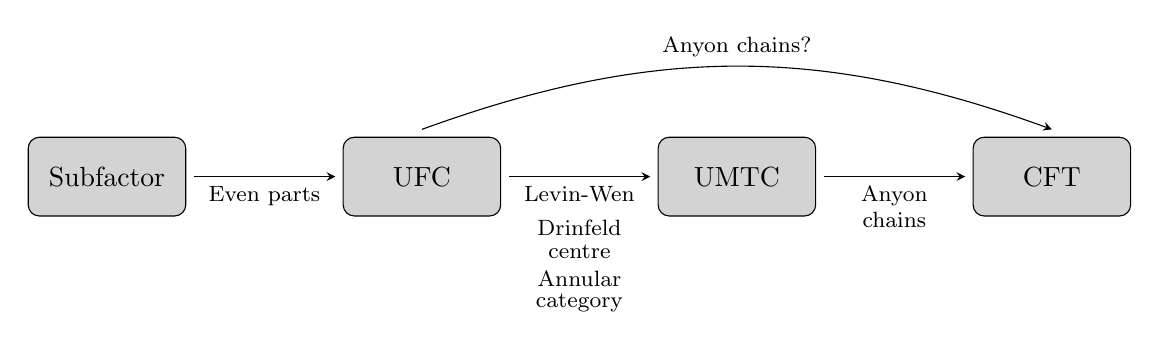
\begin{tikzpicture}
	\draw[->,>=stealth] (2.1,0.5) to node [below] {\footnotesize Even parts} (3.9,0.5);
	\draw[->,>=stealth] (6.1,0.5) to node [below] {\footnotesize Levin-Wen} (7.9,0.5);
	\draw[->,>=stealth] (5,1.1) to [bend left=20] node [above] {\footnotesize Anyon chains?} (13,1.1);
	\node at (7,-0.15) {\footnotesize Drinfeld};
	\node at (7,-0.45) {\footnotesize centre};
	\node at (7,-0.8) {\footnotesize Annular};
	\node at (7,-1.1) {\footnotesize category};
	\draw[->,>=stealth] (10.1,0.5) to node [below] {\footnotesize Anyon} (11.9,0.5);
	\node at (11,-0.05) {\footnotesize chains};
	\draw[fill=LightGray,rounded corners] (0,0) rectangle (2,1);
	\node at (1,0.5) {Subfactor};		
	\draw[fill=LightGray,rounded corners] (4,0) rectangle (6,1);
	\node at (5,0.5) {UFC};
	\draw[fill=LightGray,rounded corners] (8,0) rectangle (10,1);
	\node at (9,0.5) {UMTC};
	\draw[fill=LightGray,rounded corners] (12,0) rectangle (14,1);
	\node at (13,0.5) {CFT};
	\end{tikzpicture}
	\caption{\small \label{fig:path}\textbf{The path from subfactors to CFTs.} From a subfactor, one can get two unitary fusion categories (UFCs) via its even parts. Using one of several methods, it is possible to construct the corresponding Unitary Modular Tensor Category (UMTC). Since a UMTC describes anyons, we can build an anyon chain from it and thereby get information about the corresponding Conformal Field Theory (CFT). Building an anyon chain directly from the UFC is simpler than constructing the UMTC first, but it is not guaranteed to succeed.}
\end{figure}

A UMTC is the mathematical model for exotic quasiparticles called \emph{anyons}, which only arise in two-dimensional systems. Their statistical behaviour is much less restricted than those of the commonly known fermions and bosons, which originates from the different topologies of space-time evolutions of point-like particles in two and three dimensions: Consider the process of exchanging two indistinguishable particles as depicted in \cref{fig:anyons}. In three dimensions, the path $C_1$ that describes how one particle encircles the other, can always be continuously deformed to the path $C_2$, which does not encircle the other particle. This path in turn is contractible to a point, denoted $0$, hence the wave function of the system must satisfy
	\begin{equation}
		\Psi(C_1)=\Psi(C_2)=\Psi(0).
	\end{equation}
The process of one particle encircling the other is equivalent to exchanging the two particles twice. Hence, the evolution of the system can be represented by the exchange operator $R$ such that $\Psi(C_1)=R^2\Psi(0)$. Since $C_1$ can be contracted to a point, the exchange operator has to fulfil $R^2=1$. This has only two solutions, $R=+1$ (which corresponds to bosons) and $R=-1$ (which corresponds to fermions). In two dimensions, however, the situation is different: Here, the path $C_1$ cannot be continuously deformed to $C_2$ since it cannot cross the particle. Therefore, the exchange operator $R$ is not required to square to the identity but can be represented by a complex phase or even by a unitary matrix. In the first case, the anyons are called \emph{abelian} and in the second case \emph{non-abelian} (which comes from the fact that matrices, in general, do not commute). These exotic exchange properties can be exploited to implement quantum gates and thus realising topological quantum computation. The fact that the statistics only rely on the topological properties of the system make this approach inherently robust to environmental noise.

There is a remarkable relation between these exotic particles and conformal field theories, which we exploit to draw the final part of the connection between subfactors and CFTs. By building a one-dimensional chain of anyons with nearest-neighbour interactions, it is possible to extract information about the corresponding CFT by studying phase transitions of the system. If the model exhibits a quantum phase transition, we will observe that the correlation length diverges (when the system size goes to infinity), and with it the entanglement entropy of the system. This relation allows us, for example, to get an estimate for the \emph{central charge}, which is an important characteristic of a CFT. This approach was successfully carried out for Fibonacci anyons \cite{feiguin_interacting_2007} and for $SO(5)_2$ anyons \cite{Finch2014}. 

\begin{figure}[t]
	\begin{tikzpicture}[scale=1]
	\node at (-0.5,2.1) {\textbf{3D}};
	\begin{scope}[scale=0.8]
	\draw[->,>=stealth] (0,0) -- (1,0);
	\draw[->,>=stealth] (0,0) -- (0,1);
	\draw[->,>=stealth] (0,0) -- (225:0.7071);
	\end{scope}
	\draw[->-] (0.75,1.25) arc (180:-180:0.75cm and 0.4cm);
	\draw[->-] (0.75,1.25) arc (180:-180:1.5cm and 0.6cm);
	\shade[ball color = LinkColor!90, opacity = 1] (0.75,1.25) circle (0.25cm);
	\shade[ball color = LinkColor!90, opacity = 1] (3,1.25) circle (0.25cm);
	\node at (4,1.5) {$C_1$};
	\node at (2.45,1.5) {$C_2$};
	\end{tikzpicture}\hspace{15pt}
	\begin{tikzpicture}[scale=1]
	\node at (-0.75,2.25) {\textbf{2D}};
	\draw[fill=LightGray,LightGray] (-0.75,-0.25) -- (4,-0.25) -- (5.5,2.25) -- (0.75,2.25) -- cycle;
	\begin{scope}[scale=0.8,xshift=-0.45cm,yshift=0cm]
	\draw[->,>=stealth] (0,0) -- (1,0);
	\draw[->,>=stealth] (0,0) -- (58:0.7071);
	\end{scope}
	\draw[->-] (0.75,1.25) arc (180:-180:0.75cm and 0.4cm);
	\draw[->-] (0.75,1.25) arc (180:-180:1.5cm and 0.6cm);
	\draw[fill=LinkColor!90,LinkColor!90] (0.75,1.25) ellipse (0.25cm and 0.18cm);
	\draw[fill=LinkColor!90,LinkColor!90] (3,1.25) ellipse (0.25cm and 0.18cm);
	\node at (4,1.5) {$C_1$};
	\node at (2.45,1.5) {$C_2$};
	\end{tikzpicture}
	\caption{\small \label{fig:anyons}\textbf{Topological differences between three- and two-dimensional particle circulation.} In three dimensions, the loop $C_1$ can always be continuously deformed to the path $C_2$, which in turn is contractible to a point. In two dimensions, the paths are topologically distinct: $C_1$ cannot be continuously deformed into $C_2$.}
\end{figure}

In this thesis, we address several of the stages that are depicted in \cref{fig:path} for the example of the Haagerup subfactor. The first step is easy in this case since the two unitary fusion categories coming from the Haagerup subfactor, denoted $\Hi_1$ and $\Hi_2$, have already been constructed. Moreover, as described in \cref{ch:Haagerup}, all categories in the Morita equivalence class (which is a certain equivalence between categories) are known: Apart from the two UFCs that directly come from the subfactor, there is a third one in the Morita equivalence class, denoted $\Hd$, which is not equivalent to either of the two (only \emph{Morita equivalent}--this is an important difference). Since one characteristic of Morita equivalence is that the Drinfeld centre of the categories are equal, we can do the UMTC construction for any of the three categories. Here, the category $\Hd$ is especially easy for calculations since it is not only a fusion category but also a \emph{trivalent category}. As such, the graphical calculus within the category is particularly simple, as explained in \cref{ch:Trivalent}. However, in order to do graphical calculations within the category it is crucial to calculate the $F$\emph{-symbols}, which is done in \cref{ch:Haagerup}.

The second step, constructing the UMTC from the UFC, is more complicated. As mentioned above, the direct construction of the Drinfeld centre via its definition is an extraordinarily lengthy and complicated calculation (see \cref{sec:Drinfeld}). Another approach via the so-called tube algebra is briefly mentioned in \cref{ch:defects}, but not pursued further since it is computationally very involved. In \cref{ch:defects}, we make a slight detour from our journey from subfactors to CFTs by studying defects in spin chains. Although this does not directly contribute to answering the central question of this thesis, it is a natural generalisation of anyon chains and yields insight into the study of topological phases. Here, we also encounter the so-called \emph{annular category}, whose representations are connected to the Drinfeld centre. For the purpose of finding the UMTC, the most promising approach is the Levin-Wen model, even though it has its own unique challenges: The original model can only be constructed from UFCs that fulfil a certain symmetry condition, the so-called \emph{tetrahedral symmetry}, which is not fulfilled for the Haagerup fusion categories. Hence, the first step here is to find a generalisation of this model that also includes categories without tetrahedral symmetry, which is presented in \cref{ch:LW}. It turns out that in the general Levin-Wen model, finding the excitations is a more complicated task because of the lack of some symmetries. However, there is a promising approach of finding the excitations by constructing a tensor-network representation of the ground state of the model.

Since the possible ways of constructing the Drinfeld centre of the UFCs all involve challenging tasks and time-consuming calculations, it is worth trying a simpler approach first: Although it is not guaranteed to succeed, it is possible to build an anyon chain from the UFC directly instead of using the UMTC. Hence, in \cref{sec:anyons}, we construct the anyon chain from the category $\Hd$ and numerically study the behaviour of the ground state. Unfortunately, we find that using the UFC directly does not give rise to a quantum phase transition, hence it is inevitable that we must construct the UMTC in order to study the connection to the CFT.

This thesis is organized in two parts: In the first part, we introduce the mathematical concepts that are essential for building physical models from fusion categories. Here, we begin with an introduction to the basic concepts of category theory in \cref{ch:cats} and introduce the special case of trivalent categories in \cref{ch:Trivalent}. We then give the basic concepts of the theory of subfactors in \cref{ch:subfactor} with an emphasis on the connection to fusion categories. The final chapter of Part 1, \cref{ch:Haagerup}, discusses the Haagerup subfactor in detail and presents the corresponding fusion categories, especially the category $\Hd$, which is the motivating example of this thesis.

In the second part of this thesis we discuss several microscopic models which are built from fusion categories. We begin with describing anyon chains in \cref{sec:anyons} and present several numerical results for a chain built from the fusion category $\Hd$. In \cref{ch:defects}, we extend this concept by allowing defects to be part of this chain. We study this model for the category $\mathbf{Vec}(\mathbb{Z}/2\mathbb{Z})$. A model that connects fusion categories directly to their quantum double is the Levin-Wen model, which is discussed in \cref{ch:LW}. Here, we present a modification to the original model such that it is applicable to the category $\Hd$. Finally, we summarize the results of this thesis in \cref{ch:conclusion} and discuss potential further directions for future research.